\chapter{信号传播：行波与驻波}\label{ch:b1:wave-propagation}

拨动一根吉他弦，整个大厅都能听到这个音；
用手指轻触弦的中点，音高便升高一个八度。站在两只
放出同一音调的扬声器之间，慢慢走动，
每隔几分米便会经过一处几乎无声的位置。两个针孔
射出的光在屏幕上映出条纹。这些现象中，
任何东西都不会从一处运到另一处——空气、琴弦与玻璃都不迁移，
然而传播的是\emph{信号}。本章讨论信号如何传播，
正弦波是什么，以及两列波相遇时会发生什么：
叠加、干涉与驻波的数学，这些内容
将被此后各波动章节——声学、光学与量子物理——
反复使用。

\begin{omfigure}
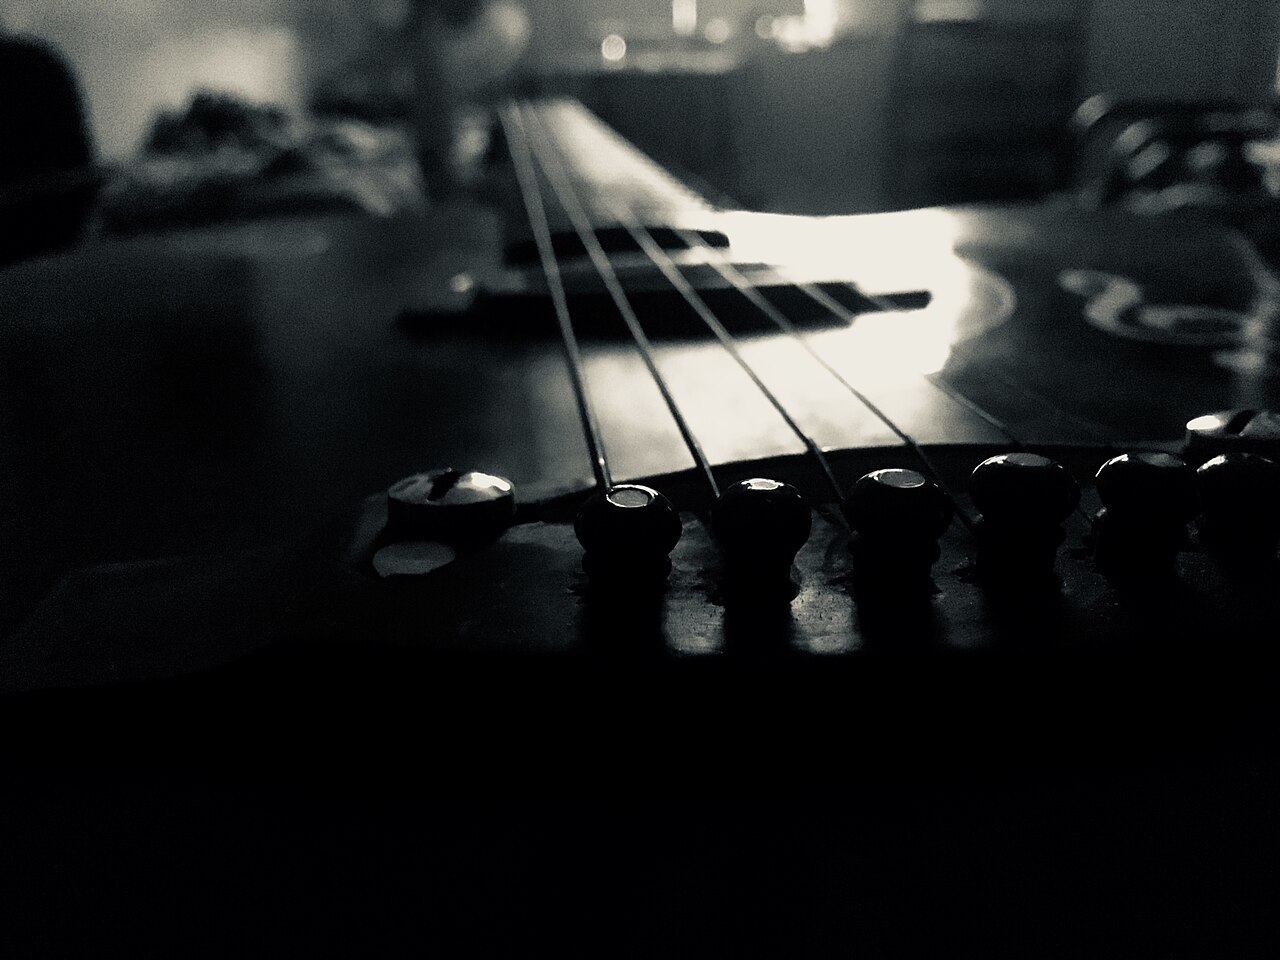
\includegraphics[width=0.55\linewidth]{images/book3/guitar-closeup.jpg}

{\small 六根弦，六个基频：每根弦都是两端固定于琴枕与琴桥之间的驻波，手指按弦可缩短弦长以提高音调。}
\end{omfigure}

\section{信号}

\begin{definition}[信号；正弦信号]\label{def:b1:wave-propagation:signal}
\index{信号}\index{正弦信号}\index{振幅}\index{相位}\index{角频率}
\emph{信号}是随时间变化并携带信息的物理量，例如
传声器处的声超压、天线处的电压、
或弦上某点的横向位移。
\emph{正弦信号}为
\[
s(t) = A\cos(\omega t + \varphi)
\]
其\emph{振幅}为 $A > 0$，\emph{角频率}为 $\omega$
（\unit{rad/s}），\emph{频率}为 $f = \omega/2\pi$，\emph{周期}
为 $T = 1/f$，\emph{初相位}为 $\varphi$；$\omega t + \varphi$ 是
时刻 $t$ 的\emph{相位}。
\end{definition}

\begin{remark}[频谱]\label{rem:b1:wave-propagation:spectrum}
\index{频谱!信号的}\index{谐波}
任一周期为 $T$ 的周期信号，都可表示为若干正弦信号之和，其频率为
$f_1 = 1/T$（\emph{基频}）及其整数倍 $nf_1$（
\emph{谐波}）；它们的振幅列表即为该信号的
\emph{频谱}。同一音高的长笛与小提琴共享
基频，但频谱不同——这就是音色。
傅里叶分解在
\cref{ch:b1:filters-transfer-functions}中陈述并使用；此处之所以重要，是因为
正弦信号的传播十分简单，对每个正弦信号成立的结论，
经叠加后对任意信号亦成立。
\end{remark}

\begin{proposition}[拍]\label{prop:b1:wave-propagation:beats}
\index{拍}
两个振幅相等、频率相近的正弦信号之和，
$f_1 > f_2$,
\[
A\cos(2\pi f_1 t) + A\cos(2\pi f_2 t)
= 2A\cos\!\big(2\pi\tfrac{f_1 - f_2}{2}\,t\big)\cos\!\big(2\pi\tfrac{f_1 + f_2}{2}\,t\big),
\]
是频率为平均值的正弦信号，其振幅为
$\abs{2A\cos(\pi(f_1 - f_2)t)}$，以\emph{拍
频}$f_1 - f_2$ 忽强忽弱。
\end{proposition}

\begin{proof}
$\cos a + \cos b = 2\cos\frac{a - b}{2}\cos\frac{a + b}{2}$。慢因子
在其自身周期 $2/(f_1 - f_2)$ 内两次为零，故
包络 $\abs{\cdot}$ 的频率为 $f_1 - f_2$。
\end{proof}

\begin{omfigure}
\begin{tikzpicture}
\begin{axis}[omaxis, axis x line=bottom, width=11.5cm, height=4.6cm, xlabel={$t$ (\unit{s})},
    ylabel={$s$}, xmin=0, xmax=1, ymin=-2.3, ymax=2.3, ytick={-2,0,2},
    yticklabels={$-2A$,$0$,$2A$}, xtick={0,0.25,0.5,0.75,1}]
  \addplot[omDef, thick, domain=0:1, samples=700] {cos(deg(2*pi*22*x)) + cos(deg(2*pi*20*x))};
  \addplot[omThm, thick, dashed, domain=0:1, samples=200] {2*cos(deg(2*pi*1*x))};
  \addplot[omThm, thick, dashed, domain=0:1, samples=200] {-2*cos(deg(2*pi*1*x))};
\end{axis}
\end{tikzpicture}

{\small 在 \qty{22}{Hz} 与 \qty{20}{Hz} 之间的拍：一个 \qty{21}{Hz}
的振动，其包络（虚线）每秒起伏两次——即
两频率之差。}
\end{omfigure}

\begin{example}[凭耳朵调音]\label{ex:b1:wave-propagation:tuning}
一只 \qty{440}{Hz} 的音叉与一根 \qty{443}{Hz} 的弦同时发声，
每秒拍动三次；拧紧弦会使拍动变慢，
拍动停止时，弦便调准了。耳朵将平均
频率（\qty{441.5}{Hz}）听作音调，并把 \qty{3}{Hz} 的包络听作
响度的起伏：拍使频率之差不足百分之一
也能被听出。
\end{example}

\section{行波}

\begin{definition}[行波；波速]\label{def:b1:wave-propagation:travelling}
\index{行波}\index{波速}\index{非色散介质}
沿某坐标轴定义的信号 $s(x, t)$ 称为\emph{行波}，
其沿 $+x$ 方向以\emph{波速} $c$ 传播，若
\[
s(x, t) = f\!\left(t - \frac{x}{c}\right) = F(x - ct)
\]
对某个函数 $f$（或 $F$）成立：波形保持不变地随之
平移了 $c\,\Delta t$，历时 $\Delta t$。沿 $-x$ 方向传播的波为
$g(t + x/c)$。若某介质中每种形状都以
相同的 $c$ 无畸变地传播，则该介质称为\emph{非色散的}。
\end{definition}

\begin{proposition}[延迟]\label{prop:b1:wave-propagation:delay}
在 $x_2$ 处接收到的信号，即在 $x_1 < x_2$ 处发出的信号，
延迟了 $\tau = (x_2 - x_1)/c$：$s(x_2, t) = s(x_1, t - \tau)$。
\end{proposition}

\begin{proof}
$s(x_2, t) = f(t - x_2/c) = f\big((t - \tau) - x_1/c\big) = s(x_1, t - \tau)$.
\end{proof}

\begin{example}[波速]\label{ex:b1:wave-propagation:celerities}
空气中的声音速率为 \qty{340}{m/s}：闪电后 \qty{3}{s} 才听到雷声，
可知雷击发生在 \qty{1}{km} 外。水中声速为 \qty{1500}{m/s}；钢中
声速为 \qty{5000}{m/s}。张力为 $F$、单位长度质量为
$\mu$ 的弦上横波：$c = \sqrt{F/\mu}$，
与量纲分析的预言一致（\cref{exo:b1:units-dimensions:5}）——吉他弦的
波速为 \qty{140}{m/s}。真空中光速 $c = \qty{3.00e8}{m/s}$；玻璃中为
$c/n$。波速是介质的性质，而非波源的性质：
耳语与大喊同时到达。
\end{example}

\begin{proposition}[正弦行波]\label{prop:b1:wave-propagation:sinusoidal}
\index{波长}\index{波数}\index{相速度}\index{双重周期性}
一个正弦波源 $s(0, t) = A\cos(\omega t)$ 发出
\[
s(x, t) = A\cos\!\big(\omega(t - x/c)\big) = A\cos(\omega t - kx),
\qquad k = \frac{\omega}{c} = \frac{2\pi}{\lambda},
\qquad \lambda = cT = \frac{c}{f}.
\]
该波在时间上以周期 $T$ 重复，在空间上以
\emph{波长} $\lambda$ 为周期；$k$ 称为\emph{波数}。相距
$d$ 的两点振动的相位差为
$\Delta\varphi = 2\pi d/\lambda = kd$：$d = n\lambda$ 时同相，
$d = (n + \tfrac12)\lambda$ 时反相。波峰移动的速率
$v_\varphi = \omega/k$ 称为\emph{相速度}；
此时 $v_\varphi = c$。
\end{proposition}

\begin{proof}
将 $f(u) = A\cos(\omega u)$ 代入 $f(t - x/c)$。固定 $x$ 时
信号经 $T = 2\pi/\omega$ 后重复；固定 $t$ 时，信号经
$\lambda$ 后重复，且 $k\lambda = 2\pi$。取两点 $x_1$、$x_2 = x_1 + d$，则
相位差为 $kd$。波峰（$\omega t - kx = \text{常数}$）的移动速度为
$\dd x/\dd t = \omega/k$.
\end{proof}

\begin{omfigure}
\begin{tikzpicture}
\begin{axis}[omaxis, width=7.2cm, height=4.2cm, xlabel={$x$}, ylabel={$s(x, t_0)$},
    xmin=0, xmax=6.5, ymin=-1.4, ymax=1.6, ytick={-1,0,1}, yticklabels={$-A$,$0$,$A$},
    xtick={0,2,4,6}, xticklabels={$0$,$\lambda$,$2\lambda$,$3\lambda$}]
  \addplot[omDef, thick, domain=0:6.5, samples=200] {cos(deg(pi*x))};
  \draw[Stealth-Stealth, omThm] (axis cs:2,1.2) -- (axis cs:4,1.2) node[midway, above, font=\footnotesize] {$\lambda$};
  \draw[-Stealth, omExo, thick] (axis cs:4.7,1.2) -- (axis cs:5.7,1.2) node[midway, above, font=\footnotesize] {$c$};
\end{axis}
\end{tikzpicture}\qquad
\begin{tikzpicture}
\begin{axis}[omaxis, width=7.2cm, height=4.2cm, xlabel={$t$}, ylabel={$s(x_0, t)$},
    xmin=0, xmax=6.5, ymin=-1.4, ymax=1.6, ytick={-1,0,1}, yticklabels={$-A$,$0$,$A$},
    xtick={0,2,4,6}, xticklabels={$0$,$T$,$2T$,$3T$}]
  \addplot[omDef, thick, domain=0:6.5, samples=200] {cos(deg(pi*x))};
  \draw[Stealth-Stealth, omThm] (axis cs:2,1.2) -- (axis cs:4,1.2) node[midway, above, font=\footnotesize] {$T$};
\end{axis}
\end{tikzpicture}

{\small 正弦行波的双重周期性：
固定时刻的快照每隔一个波长 $\lambda$ 重复一次，并以
速率 $c$ 平移；某固定点处的信号每隔一个周期 $T$ 重复，
且 $\lambda = cT$。}
\end{omfigure}

\begin{definition}[色散]\label{def:b1:wave-propagation:dispersion}
\index{色散介质}
若相速度随频率而变，则称该介质为\emph{色散的}。非正弦信号，
即若干正弦之和，在传播中会变形，各分量彼此分开。
空气中的声音与真空中的光都是非色散的；玻璃中的光
（见\cref{ch:b1:rays-reflection-refraction}）与深水波都是色散的——
远方风暴的长涌浪
比近处的短碎浪早一天到达。
\end{definition}

\section{叠加与干涉}

\begin{theorem}[叠加原理]\label{thm:b1:wave-propagation:superposition}
\index{叠加原理}
在线性介质中，若干波同时传播时，
每一点、每一时刻的合成信号，
等于各波单独传播时所产生的信号之和。
\end{theorem}
\admitted

\begin{remark}[线性]\label{rem:b1:wave-propagation:linearity}
叠加性是关于介质方程的结论（方程关于信号是线性的），
只要振幅保持较小便成立：低于痛阈的声音、低于激光切割强度的光、
轻轻拨动的弦。两束光可以交叉而互不影响；
两列涟漪相互穿过，且各自保持完整。
在\emph{重叠之处}所观察到的现象，
正是干涉的研究对象。
\end{remark}

\begin{theorem}[同频率的两个正弦信号]\label{thm:b1:wave-propagation:fresnel}
\index{干涉}\index{菲涅耳公式}\index{相长干涉}\index{相消干涉}
在某点处，若有两个同频率的正弦信号到达，
$s_1 = A_1\cos(\omega t + \varphi_1)$ 与 $s_2 = A_2\cos(\omega t + \varphi_2)$，
二者之和是同频率的正弦信号，其振幅满足
\[
A^2 = A_1^2 + A_2^2 + 2A_1A_2\cos\Delta\varphi,
\qquad \Delta\varphi = \varphi_2 - \varphi_1 .
\]
对于强度（单位面积上的功率）正比于
$A^2$ 的波，其强度服从\emph{菲涅耳公式}
\[
I = I_1 + I_2 + 2\sqrt{I_1 I_2}\,\cos\Delta\varphi .
\]
干涉为\emph{相长的}（$A = A_1 + A_2$），条件是
$\Delta\varphi = 2n\pi$；干涉为\emph{相消的}（$A = \abs{A_1 - A_2}$），条件是
$\Delta\varphi = (2n + 1)\pi$，$n \in \Z$。
\end{theorem}

\begin{proof}
展开：$s_1 + s_2 = (A_1\cos\varphi_1 + A_2\cos\varphi_2)\cos\omega t -
(A_1\sin\varphi_1 + A_2\sin\varphi_2)\sin\omega t = X\cos\omega t -
Y\sin\omega t = A\cos(\omega t + \varphi)$ 其中 $A^2 = X^2 + Y^2 =
A_1^2 + A_2^2 + 2A_1A_2(\cos\varphi_1\cos\varphi_2 + \sin\varphi_1\sin\varphi_2)$。
几何上，$A$ 为两矢量之和的长度，这两矢量的长度分别为
$A_1$、$A_2$，夹角为 $\Delta\varphi$（余弦定理）。
\end{proof}

\begin{proposition}[同相的两个波源；光程差]\label{prop:b1:wave-propagation:pathdiff}
\index{光程差}
两个同相发射、波长为 $\lambda$ 的波源，
$d_1$、$d_2$ 分别是两波源到点 $M$ 的距离，两波到达 $M$ 时的相位差为
$\Delta\varphi = 2\pi\,\delta/\lambda$，其中 $\delta = d_2 - d_1$ 称为
\emph{光程差}。点 $M$ 处的干涉，相长的条件是
$\delta = n\lambda$，相消的条件是 $\delta = (n + \tfrac12)\lambda$。
\end{proposition}

\begin{proof}
每列波到达时带有其传播路程引起的相位滞后 $kd_i = 2\pi d_i/\lambda$
（见\cref{prop:b1:wave-propagation:sinusoidal}）；两者之差为
$2\pi(d_2 - d_1)/\lambda$。运用\cref{thm:b1:wave-propagation:fresnel}。
\end{proof}

\begin{example}[两个扬声器]\label{ex:b1:wave-propagation:speakers}
两个扬声器相距 \qty{2.0}{m}，发出相同的 \qty{850}{Hz} 纯音，
且同相（$\lambda = \qty{0.40}{m}$）。在中垂线上
$\delta = 0$ 处处都响。沿两扬声器的连线，位移每增加一个波长，$\delta$
改变 $2\lambda$，因此安静点
（$\delta = \pm\lambda/2, \pm 3\lambda/2, \dots$）每隔
$\lambda/2 = \qty{20}{cm}$ 出现一处——这是驻波，
即下一节的主题。将一只扬声器的接线对调，使其反相发声，则
响处与静处互换。
\end{example}

\begin{example}[杨氏双孔]\label{ex:b1:wave-propagation:young}
\index{杨氏双孔}\index{条纹间距}\index{光程}
两个针孔 $S_1$、$S_2$ 相距 $a$，由一个单色光源照明，
（使二者同相发射），射向一块屏幕，
屏幕距离为 $D \gg a$。屏上距轴线高度为 $x$ 的一点处，
光程差为
\[
\delta = S_2M - S_1M \approx \frac{a\,x}{D}
\]
（当 $x \ll D$ 时：$S_{1,2}M = \sqrt{D^2 + (x \mp a/2)^2} \approx D +
(x \mp a/2)^2/2D$，再相减）。亮条纹位于 $x = n\lambda D/a$ 处，
\emph{条纹间距}为
\[
i = \frac{\lambda D}{a} .
\]
已知 $a = \qty{0.50}{mm}$，$D = \qty{2.0}{m}$，$\lambda = \qty{633}{nm}$：
$i = \qty{2.5}{mm}$——用一把尺子即可测出光的波长。在
折射率为 $n$ 的介质中，计算光程差应使用
\emph{光程}，即 $n \times$ 长度，因为 $\lambda = \lambda_0/n$。
\end{example}

\begin{omfigure}
\begin{tikzpicture}[font=\small, x=1cm, y=1cm]
  \fill (0,0.4) circle (1.5pt) node[left] {$S_1$};
  \fill (0,-0.4) circle (1.5pt) node[left] {$S_2$};
  \draw[Stealth-Stealth] (-0.9,0.4) -- (-0.9,-0.4) node[midway, left] {$a$};
  \draw[thick] (5.6,-2.2) -- (5.6,2.2); \node[above] at (5.6,2.2) {屏};
  \fill[omThm] (5.6,1.3) circle (1.5pt) node[right] {$M$};
  \draw[omDef] (0,0.4) -- (5.6,1.3); \draw[omDef] (0,-0.4) -- (5.6,1.3);
  \draw[dashed] (0,0) -- (5.6,0) node[below right] {$O$};
  \draw[Stealth-Stealth] (5.9,0) -- (5.9,1.3) node[midway, right] {$x$};
  \draw[Stealth-Stealth] (0,-2.0) -- (5.6,-2.0) node[midway, below] {$D$};
  \node[omDef] at (2.8,1.2) {$d_1$}; \node[omDef] at (3.3,0.28) {$d_2$};
  % fringes pattern
  \begin{scope}[xshift=7.6cm]
  \begin{axis}[omaxis, axis x line=bottom, width=4.2cm, height=5.2cm, xlabel={$I$}, ylabel={$x$},
      xmin=0, xmax=4.6, ymin=-2.2, ymax=2.2, xtick={0,4}, xticklabels={$0$,$4I_0$},
      ytick={-2,-1,0,1,2}, yticklabels={$-2i$,$-i$,$0$,$i$,$2i$}, anchor=origin, at={(0,0)}]
    \addplot[omThm, thick, domain=-2.2:2.2, samples=300] ({4*cos(deg(pi*x))^2},{x});
  \end{axis}
  \end{scope}
\end{tikzpicture}

{\small 杨氏双孔：两个同相波源，相距 $a$，
沿路径到达远处屏上的点 $M$，二者路径差为
$\delta \approx ax/D$。屏上光强为 $4I_0\cos^2(\pi x/i)$，
明暗条纹交替出现，条纹间距为 $i = \lambda D/a$。}
\end{omfigure}

\begin{remark}[相干性]\label{rem:b1:wave-propagation:coherence}
\index{相干性}
菲涅耳公式假设相位差固定。两盏独立的灯
各自的相位每秒随机跳变数十亿次；
$\cos\Delta\varphi$ 的平均值为零，因此光强只是简单相加，
没有条纹。干涉需要\emph{相干的}波源——实际上，
即同一光源发出的两列波，经两个小孔、两条狭缝、薄膜的两个表面，
或分束器分出的两列波。由同一信号发生器驱动的两个扬声器
是相干的；两位歌手则不是。
\end{remark}

\section{驻波}

\begin{theorem}[驻波]\label{thm:b1:wave-propagation:standing}
\index{驻波}\index{波节}\index{波腹}
振幅和频率均相同的两列正弦波，沿
相反方向传播，叠加为
\[
A\cos(\omega t - kx) + A\cos(\omega t + kx) = 2A\cos(kx)\cos(\omega t),
\]
这是\emph{驻波}：每一点都同相（或反相）
振动，振幅为 $2A\abs{\cos kx}$，随位置变化——
在\emph{波节}（$x = (n + \tfrac12)\lambda/2$）处为零，在
\emph{波腹}（$x = n\lambda/2$）处最大；相邻波节相距 $\lambda/2$。驻波
中不存在波的传播：变量 $x$ 与 $t$ 已分离。
\end{theorem}

\begin{proof}
$\cos a + \cos b = 2\cos\frac{a - b}{2}\cos\frac{a + b}{2}$，其中
$a = \omega t - kx$，$b = \omega t + kx$。
\end{proof}

\begin{proposition}[两端固定弦的模式]\label{prop:b1:wave-propagation:modes}
\index{模式（本征模）}\index{基频}\index{梅尔德实验}
长为 $L$、波速为 $c$、在 $x = 0$ 与 $x = L$ 处固定的弦，
只有当 $L$ 恰为整数个
半波长时，才能维持正弦驻波：
\[
\lambda_n = \frac{2L}{n}, \qquad f_n = n\,\frac{c}{2L} = n f_1,
\qquad n = 1, 2, 3, \dots
\]
这些即其\emph{模式}；$f_1 = c/2L$ 为\emph{基音}，
$f_n$ 则为其各谐音。在一端以接近
$f_n$ 的频率驱动时，弦以第 $n$ 个模式的形状共振（
梅尔德实验）；拨动时，弦做多个模式的叠加振动，
耳朵听到的音调为 $f_1$。
\end{proposition}

\begin{proof}
固定端为波节。在 $x = L$ 处反射的波向回传播，
与入射波叠加成驻波；要使其
在 $x = 0$ 处亦为波节，则 $\cos kx$ 须换为 $\sin kx$（平移原点），
且 $\sin kL = 0$：$kL = n\pi$，$\lambda_n = 2L/n$，
于是 $f_n = c/\lambda_n$。
\end{proof}

\begin{omfigure}
\begin{tikzpicture}[font=\small, x=1cm, y=1cm]
  \foreach \n/\yo/\lab in {1/3.0/{$n = 1$: $\lambda_1 = 2L$, $f_1$}, 2/1.5/{$n = 2$: $\lambda_2 = L$, $2f_1$}, 3/0/{$n = 3$: $\lambda_3 = 2L/3$, $3f_1$}} {
    \draw[thick] (0,\yo-0.55) -- (0,\yo+0.55); \draw[thick] (6,\yo-0.55) -- (6,\yo+0.55);
    \draw[dashed] (0,\yo) -- (6,\yo);
    \draw[omDef, thick, domain=0:6, samples=120, variable=\x] plot ({\x},{\yo+0.5*sin(deg(\n*pi*\x/6))});
    \draw[omDef!50, thick, domain=0:6, samples=120, variable=\x] plot ({\x},{\yo-0.5*sin(deg(\n*pi*\x/6))});
    \node[right] at (6.3,\yo) {\lab};
  }
  \foreach \x in {0,3,6} {\fill[omThm] (\x,1.5) circle (1.5pt);}
  \foreach \x in {0,2,4,6} {\fill[omThm] (\x,0) circle (1.5pt);}
  \node[omThm, below] at (3,1.3) {波节};
  \node[omDef, above] at (1.5,3.55) {波腹};
  \draw[Stealth-Stealth] (0,-0.9) -- (6,-0.9) node[midway, below] {$L$};
\end{tikzpicture}

{\small 两端固定弦的前三个模式：$n$
个半波长嵌入 $L$ 之中；弦在两个极端形状（深色与浅色）之间
摆动，波节保持静止。频率 $f_n = nf_1$。}
\end{omfigure}

\begin{example}[吉他弦]\label{ex:b1:wave-propagation:guitar}
$L = \qty{65}{cm}$，调至 $f_1 = \qty{110}{Hz}$：$c = 2Lf_1 =
\qty{143}{m/s}$；取 $\mu = \qty{5.0}{g/m}$，张力为 $F = \mu c^2
= \qty{102}{N}$——相当于每根弦上挂着十千克的重物。手指
按在第十二品处，使 $L$ 减半、$f_1$ 加倍：即八度音。
手指仅\emph{触及}弦的中点，便在该处强制形成波节，
并消去所有奇次模式：弦以 $2f_1$ 发声，此即吉他手所说的
“谐音”。
\end{example}

\begin{remark}[管道，以及预告]\label{rem:b1:wave-propagation:pipes}
长笛内两端开口的空气柱，两端均为压强波节，
其模式同为 $f_n = nc/2L$；一端封闭的管子，
封闭端为波节，开口端为波腹，故
$L = (2n + 1)\lambda/4$，只有奇次谐音 $f = (2n + 1)c/4L$
能够发声——这便是单簧管空洞的音色。将波限制在两
壁之间，因而\emph{量子化}其频率；当该波为电子在原子中的物质波时，
同样的半波长计数使其能量
量子化（见\cref{ch:b1:quantum-introduction}）。
\end{remark}

\section{练习}

\begin{exercise}[$\star$]\label{exo:b1:wave-propagation:1}
雷声在闪光后 \qty{6.0}{s} 才到达：雷击处距离多远？另有
一个声呐脉冲在水中经 \qty{0.40}{s} 返回（$c = \qty{1500}{m/s}$）：
海底深度是多少？
\end{exercise}

\begin{exercise}[$\star$]\label{exo:b1:wave-propagation:2}
频率为 \qty{440}{Hz} 的声波在空气中传播（速率为 \qty{340}{m/s}）。求其波长，
沿传播方向相距 \qty{20}{cm} 的两只传声器之间的相位差，
以及两点振动同相时的
距离。
\end{exercise}

\begin{exercise}[$\star$]\label{exo:b1:wave-propagation:3}
一根弦的张力为 \qty{80}{N}，单位长度的质量为
\qty{4.0}{g/m}：求 $c$，以及该弦上频率为 \qty{200}{Hz}
的波的波长。
\end{exercise}

\begin{exercise}[$\star$]\label{exo:b1:wave-propagation:4}
一只频率为 \qty{440}{Hz} 的音叉与一根频率为 \qty{444}{Hz} 的弦同时发声：
每秒有多少次拍？包络的周期是多少？将弦
放松，拍频降至 \qty{1}{Hz}：此时弦的频率
为多少？（原则上有两个答案——哪一个？你将如何检验？）
\end{exercise}

\begin{exercise}[$\star\star$]\label{exo:b1:wave-propagation:5}
一根长 \qty{0.60}{m}、$c = \qty{240}{m/s}$ 的弦，两端
固定。求前三个模式的频率，以及第三个模式的
波节位置。弦应在何处触按，才能使其发出
\qty{600}{Hz} 的声音？
\end{exercise}

\begin{exercise}[$\star\star$]\label{exo:b1:wave-propagation:6}
两只相距 \qty{2.0}{m} 的扬声器同相发出 \qty{850}{Hz} 的声音
（$c = \qty{340}{m/s}$）。求连接二者的线段
上静音点的位置，并说明沿中垂线行走的听者
会听到什么。若其中一只扬声器接成反相，情况有何变化？
\end{exercise}

\begin{exercise}[$\star\star$]\label{exo:b1:wave-propagation:7}
杨氏双缝：$a = \qty{0.20}{mm}$，$D = \qty{1.5}{m}$，钠光
$\lambda = \qty{589}{nm}$。求条纹间距；再求
波长为 \qty{450}{nm} 的蓝光的条纹间距；用钠灯时，中心附近
\qty{2.0}{cm} 范围内可容纳多少条亮纹？
\end{exercise}

\begin{exercise}[$\star\star$]\label{exo:b1:wave-propagation:8}
两列强度分别为 $I_0$ 和 $I_0$ 的相干波发生干涉，求
$I_{\max}$ 和 $I_{\min}$。对强度分别为 $I_0$ 和 $I_0/4$ 的情形，问题相同。定义
对比度 $(I_{\max} - I_{\min})/(I_{\max} + I_{\min})$，
并在两种情形下计算它。
\end{exercise}

\begin{exercise}[$\star\star$]\label{exo:b1:wave-propagation:9}
一根长 \qty{0.50}{m} 的管子（$c = \qty{340}{m/s}$）。求其前三个
共振频率：若一端封闭；再求两端开口时的
共振频率。哪一种对应单簧管，哪一种对应长笛？
\end{exercise}

\begin{exercise}[$\star\star\star$]\label{exo:b1:wave-propagation:10}
在深水中，正弦波的相速度为
$v_\varphi = \sqrt{g\lambda/2\pi}$。分别计算 $\lambda = \qty{10}{m}$
和 \qty{100}{m} 时的相速度。远处 \qty{1000}{km} 外的风暴同时激起这两种波，哪一种涌浪
先到达海岸，早了多长时间？为何这使海面成为
“色散的”？
\end{exercise}

\begin{exercise}[$\star\star\star$]\label{exo:b1:wave-propagation:11}
证明：轻触弦线上距一端 $L/3$ 的一点，
只剩频率为 $3f_1, 6f_1, \dots$ 的模式，并证明
在中点拨弦不会激发任何偶次模式。（提示：
在该点处，波节或最大位移对每个模式的
$\sin(n\pi x/L)$ 有何要求？）
\end{exercise}

\begin{exercise}[$\star\star\star$]\label{exo:b1:wave-propagation:12}
一台收音机位于金属墙前距离 $d$ 处，接收远处发射机发出的直达波，
以及被墙面反射的波；该反射波多走 $2d$ 的路程，
并在反射时附加相位 $\pi$。
在 $f = \qty{100}{MHz}$ 时，求信号消失的距离 $d$，
以及信号最强的那些距离。这一结果如何
解释汽车收音机在隧道中的“盲区”？
\end{exercise}

\section{问题：梅尔德弦与吉他}

\begin{problem}[{周末问题——长凳上的振动弦、滑轮和一些重物，
然后是吉他：如何通过计数半波长，
来确定指板上的每一个音}]
\label{pb:b1:wave-propagation:1}
一根单位长度质量为 $\mu$ 的弦水平张紧，张力为 $F$，
一端连接位于 $x = L$ 处的小型电磁振子（它以极小的振幅、频率 $f$ 使弦横向振动），
另一端固定于 $x = 0$ 处；
弦上的横波传播速率为
$c = \sqrt{F/\mu}$（推导见本科二年级分册）。

\medskip
\noindent\textbf{第一部分——弦上的波。}
\begin{enumerate}
  \item 用量纲分析检验 $\sqrt{F/\mu}$ 是一个速率。
  \item 振子向 $x = 0$ 方向发出波
        $s_i(x, t) = A\cos(\omega t + kx)$。为何取符号 $+kx$？求 $k$
        用 $f$ 与 $c$ 表示。
  \item 已知 $\mu = \qty{1.0}{g/m}$，$F = \qty{0.90}{N}$ 且
        $f = \qty{50}{Hz}$，计算 $c$、$\lambda$ 和 $k$。
  \item 弦上两点相距 \qty{15}{cm}，
        对此行波而言，两点运动之间的
        相位差是多少？
  \item 若 $A = \qty{2.0}{mm}$，求弦上一点的最大
        横向速度，并与 $c$ 比较。
\end{enumerate}

\medskip
\noindent\textbf{第二部分——反射与驻波。}
在固定端 $x = 0$ 处，波被反射，符号相反：
$s_r(x, t) = -A\cos(\omega t - kx)$。
\begin{enumerate}[resume]
  \item 为何反射波的相位中须含 $-kx$，为何振幅须取反
        （想一想：总信号必须
        在 $x = 0$ 处为多少？）
  \item 证明 $s = s_i + s_r = -2A\sin(kx)\sin(\omega t)$。
  \item 求出波节与波腹的位置，给出相邻两个
        相邻波节之间的距离。
  \item 振子自身的振幅极小，以至 $x = L$ 处
        近似为波节。由此推出，要得到大振幅驻波（共振），
        $L$ 应满足的条件，并求允许的频率 $f_n$。
  \item 取 $L = \qty{1.20}{m}$，用第 3 题的数据，
        共出现多少个半波长（“纺锤”）？弦是否
        处于共振状态？
  \item 保持 $f = \qty{50}{Hz}$ 与 $L$ 不变，求得到
        $3$ 个与 $6$ 个“纺锤”共振所需的张力。
  \item 反过来，可通过计数“纺锤”测量 $\mu$：取
        $F = \qty{1.6}{N}$，频率 \qty{50}{Hz}，长 \qty{1.20}{m} 的弦上出现 $3$ 个“纺锤”，
        求 $\mu$。
  \item 张力由悬挂于滑轮上的质量 $m$ 设定，
        $F = mg$，$m$ 为 \qty{163}{g}，精确到 $\pm\qty{1}{g}$，且
        $L$ 精确到 $\pm\qty{2}{mm}$。哪一项测量限制了 $\mu$，
        其相对不确定度是多少？
\end{enumerate}

\medskip
\noindent\textbf{第三部分——吉他。}
振动长度 $L = \qty{650}{mm}$ 的六根弦，分别调至
\qty{82.4}{Hz}（低音 E）、$110$、$147$、$196$、$247$ 和 \qty{329.6}{Hz}
（高音 E）。
\begin{enumerate}[resume]
  \item 耳朵把哪一种模式当作音调？将每根弦上的 $c$ 用 $L$ 与音调表示，
        并计算两根 E 弦的波速。
  \item 低音 E 弦的 $\mu = \qty{6.0}{g/m}$，高音 E 弦的
        $\mu = \qty{0.40}{g/m}$，求二者的张力。为何低音弦要用金属丝缠绕，
        而不是仅仅拉得更紧？
  \item 西方音乐将八度分为十二个相等的半音：
        每一品使频率乘以 $2^{1/12}$。证明第
        $n$ 品必位于距琴枕 $L(1 - 2^{-n/12})$ 处，
        并计算第 $1$、$5$、$7$ 和 $12$ 品的位置。
  \item 品距沿琴颈向上逐渐减小：相邻两品之间，
        间距之比是多少？
  \item 将变调夹夹在第 $3$ 品上，所有弦均缩短：
        每个音高提高为原来的多少倍，
        新的振动长度是多少？
  \item 轻触（而非按压）低音 E 弦的第 $12$ 品上方，然后
        在第 $7$ 品上方（即 $L/3$ 处）轻触，得到两个“谐音”：
        各对应什么频率？保留了哪些模式？
  \item 靠近琴桥拨弦，听起来比在音孔上方拨弦
        更明亮。结合模式形状加以解释。
  \item 两根弦调成相隔五度（$f_2 = 1.5f_1$）。同时弹奏时，
        听者会听到一个微弱的拍，拍频为 \qty{2}{Hz}，它出现在低弦的三次谐音
        与高弦的二次谐音之间。
        求实际比值 $f_2/f_1$，
        若 $f_1 = \qty{110}{Hz}$？
\end{enumerate}

\medskip
\noindent\textbf{第四部分——用音叉调音。}
\begin{enumerate}[resume]
  \item 将 A 弦（\qty{110}{Hz}）与 \qty{440}{Hz} 的
        音叉对照调音。弦的哪一次谐音与音叉产生拍？若
        每秒听到 \qty{3}{} 次拍，
        则弦的两个可能频率为多少？
  \item 转动弦轴会略微增大张力，拍频随之加快：
        两种可能中究竟是哪一种？张力须按
        多大的相对量变化，才能达到正确音高？
  \item 证明：张力的相对变化 $\dd F/F$ 使频率的相对变化为
        $\dd f/f = \tfrac12\,\dd F/F$。
  \item 总结上述结果的逻辑链：弦长、张力与
        质量如何决定其基音，琴品如何确定音阶，以及
        拍如何调音——并指出这一切背后的唯一关系。
\end{enumerate}
\end{problem}
